\begin{document}
\title{Übungsblatt~2}
\subtitle{Einführung, Dateiverwaltung}
\maketitle

\section*{Lernziele}
\begin{itemize}
	\item Ziele des Schlüsselzugriffs
	\item Hashing als Methode des Schlüsselzugriffs
	\item Wahl der Hashfunktion und Überlaufbehandlung beim Hashing
	\item Lineares Hashing
\end{itemize}


\begin{normalText}
\section*{Literatur}
\HaerderNintyNine{7.4, 7.5, 7.6}

\ElmasriSeventh{16.8}
\end{normalText}

\section{Fragen zur Vorlesung}
\begin{enumerate}[a)]
	\item Wozu dient der Datenbankpuffer?

	\begin{solution}
	Der Datenbankpuffer dient dem Zwischenspeichern von Daten im Hauptspeicher. Ziel ist es, die Performance zu erhöhen, indem man Blöcke nicht erst von der langsamen Platte lesen muss, sondern sie im schnellen Hauptspeicher vorhält.
	\end{solution}


	\item Warum verwendet man nicht einfach die Pufferverwaltung des Betriebssystems?

	\begin{solution}
	\begin{itemize}
		\item Tut man ja. Die Pufferverwaltung des BS ist weiterhin aktiv und kann Daten auf die Platte auslagern, von denen das DBMS glaubt, sie seien im Speicher.

		\item Das Betriebssystem weiß weniger über die anwendungsspezifischen Zugriffsmuster und kann daher keine optimale Strategie anwenden. Für unseren speziellen Anwendungsfall können wir es besser. Das ist der Hauptgrund, warum man sich nicht alleine auf das BS verlässt. Außerdem bietet das Betriebsystem nicht die Schnittstellen, die für die anderen Schichten gebraucht werden (z.\,B. Transaktionssystem).

		\begin{note}
		\item Weitere Überlegung (technisch, müssen die Teilnehmer nicht wissen): Die Pufferverwaltung des BS stellt jedem Programm einen (virtuellen) Adressraum zur Verfügung, den dieses nutzen kann. Es kann dann Seiten dieses virtuellen Adressraumes an beliebige Stellen des physischen Adressraumes schieben oder sie gar auf die Platte auslagern. Die Anwendung sieht davon nichts, sie greift einfach auf Adressen im virtuellen Adressraum zu. In unserem Fall hieße das, wir würden die gesamte Datenbank in den virtuellen Adressraum kopieren und das BS entscheiden lassen, welche Frames/Seiten davon wirklich im Hauptspeicher liegen. Dank \texttt{mmap()} o.\,ä. geht das sogar schnell. Allerdings ist bei 32-bit-Architekturen der Adressraum auf 4\,GiB beschränkt, das ist viel zu wenig. Unter 64-bit Linux stehen pro
Prozess 128\,TiB virtueller Adressraum zur Verfügung, unter 64-bit Windows 8\,TiB. Auch das kann von großen Datenbanken überschritten werden. Man muss also entscheiden, welche Frames im virtuellen Adressraum liegen sollen. Und das ist bereits wieder eine eigene Pufferverwaltung.
		\end{note}
	\end{itemize}
	\end{solution}


	\item Welche Probleme kann ein Puffer im Fehlerfall (z.\,B. Stromausfall) verursachen? Wie kann man damit umgehen?

	\begin{solution}
	Wenn nicht gespeicherte Änderungen im Puffer liegen, gehen sie verloren. Das ist nicht zu ändern und immer unangenehm, besonders aber wenn Inkonsistenzen auftreten.

	Beispiele:
	\begin{itemize}
		\item Änderungen in verzweigten Strukturen (Listen Element verschieben, B-Baum-Splitt): Nachfolger sind schon persistiert, Vorgänger noch nicht $\rightarrow$ es fehlt die Verzweigung, der Nachfolger kann nicht gefunden werden.
		\item Freispeicherverwaltung (vgl. Übung 4 -- Sätze): Ein Satz wurde in einen Block eingefügt, die Freispeichertabelle ist noch nicht angepasst.
		\item Wir überweisen Geld. Abbuchung ist schon auf der Platte, Gutschrift noch nicht $\rightarrow$ Geldvernichtung
	\end{itemize}
	Minimalziel ist es daher immer, einen konsistenten Zustand zu gewährleisten. Ab da können die Anwendungen ihre Arbeit ggf. noch mal machen. Das schafft man z.B. indem man alte Blöcke nicht überschreibt, sondern den neuen Inhalt in neue Blöcke schreibt und atomar umschaltet.

	Bei den ersten beiden Beispielen, weiß das DBMS, welche Änderungen zusammengehören und wieder zu einem konsistenten Zustand führen. Im dritten Beispiel weiß das nur die Anwendung $\rightarrow$ Transaktionen, siehe später
	\end{solution}


	\item Was ist der Unterschied zwischen direkter und indirekter Seitenzuordnung? Was ist der Unterschied zwischen direkter und indirekter Seiteneinbringung?

	\begin{solution}

	\paragraph{Block, Seite und Kachel}
	Zunächst unterscheiden wir die Begriffe Block, Seite und Kachel:
	\begin{description}
		\item[Block] Block auf der physischen Festplatte, es werden immer ganze Blöcke gelesen und geschrieben und von der Platte in den Hauptspeicher transportiert und umgekehrt.
		\item[Kachel] Eine Kachel ist der Platz für einen Block im Datenbankpuffer. %% im (virtuellen) Hauptspeicher
		\item[Seite] Eine Seite ist die Adressierungseinheit an der Pufferschnittstelle. Eine Seite wird auf Blöcke abgebildet und ist genauso groß wie ein Block. Die höhere Softwareschicht arbeitet nur noch mit Seiten.
	\end{description}


	\paragraph{Seitenzuordnung}
	\begin{description}
		\item[Direkte Seitenzuordnung] bedeutet, dass aufeinanderfolgende Seiten auch in aufeinanderfolgenden Blöcken einer Datei abgelegt werden. Man muss sich also nur die erste Blocknummer für ein Segment merken und kann die Blocknummern für alle Seiten des Segments ausrechnen.

		Das hat nichts mit den Kacheln im Puffer zu tun. Im Puffer können die Seiten deshalb trotzdem komplett verstreut liegen und auch einzeln verdrängt werden. Der Puffer merkt sich zu jeder Kachel, welche Seite darin liegt und kann durch die Seitenzuordnung ermitteln, in welchen Block sie geschrieben werden muss.

		\item[Indirekte Seitenzuordnung] heißt, dass über eine Tabelle festgelegt wird, welche Seite auf welchen Block einer Datei abgebildet wird. Hintereinanderliegende Seiten müssen also nicht mehr in aufeinanderfolgenden Blöcken liegen.
	\end{description}

	Direkt ist schneller und benötigt weniger Verwaltungsdaten, dafür ist es aber auch unflexibler.

	\paragraph{Einbringstrategie}
	Die grundlegende Idee ist, dass speichern auf der Festplatte beim Verdrängen aus dem Puffer nicht notwendigerweise sofort ein Einbringen in den Datenbestand sein muss.

	\begin{description}
		\item[Direkte Seiteneinbringung] heißt, dass Seiten, die auf die Platte gespeichert werden, weil sie aus dem Puffer verdrängt werden, sofort in den Datenbestand eingebracht werden. Das heißt, alle Zeiger und Zuordnungstabellen zeigen sofort auf die neuen Daten. Das geschieht im allgemeinen einfach dadurch, dass die Seite wieder in den Block geschrieben wird, aus dem sie gelesen wurde.
		\item[Indirekte Seiteneinbringung] heißt, geänderte Seiten werden nicht sofort, wenn sie aufgrund der Verdrängung aus dem Puffer auf die Platte gespeichert werden, in den Datenbestand eingebracht. Dies geschieht erst später, z.B. nach einer Datenänderung erst dann, wenn alle Daten der Transaktion geändert sind und auch die Seiten der zugehörigen Indexstrukturen (z.B. B-Bäume) angepasst sind. Hierzu werden die verdrängten Seiten zunächst in neue Blöcke geschrieben und diese erst später durch Änderung von Verwaltungsstrukturen als zum Datenbestand gehörig gekennzeichnet.
	\end{description}

Indirekte Seiteneinbringung ist aufwändiger, bietet aber den Vorteil, dass man den alten Block im Fehlerfall wiederherstellen kann, da er ja noch existiert.
 Direkte Seiteneinbringung hingegen ist von sich aus nicht fehlertolerant. Fehlertoleranz kann z.\,B. über das Führen eines Logs erreicht werden. Die Wiederherstellung muss im Fehlerfall dann das Log auswerten und Änderungen rückgängig machen.

Die Kombination indirekter Seiteneinbringung mit direkter Seitenzuordnung wird beispielsweise durch das Twin-Slot-Verfahren (siehe VL-Folie~\TwinSlot) realisiert.
\end{solution}
\end{enumerate}


\section{Festplatten- und Flash-Laufwerke}

\subsection{Was sind Festplatten- (HDD) und Flash-Laufwerke (SSD)?}
Beschreiben Sie kurz den Aufbau von und den Zugriff auf HDDs und SSDs.

\begin{solution}
	\begin{minipage}{0.5\linewidth}
		Aufbau HDD:\\
		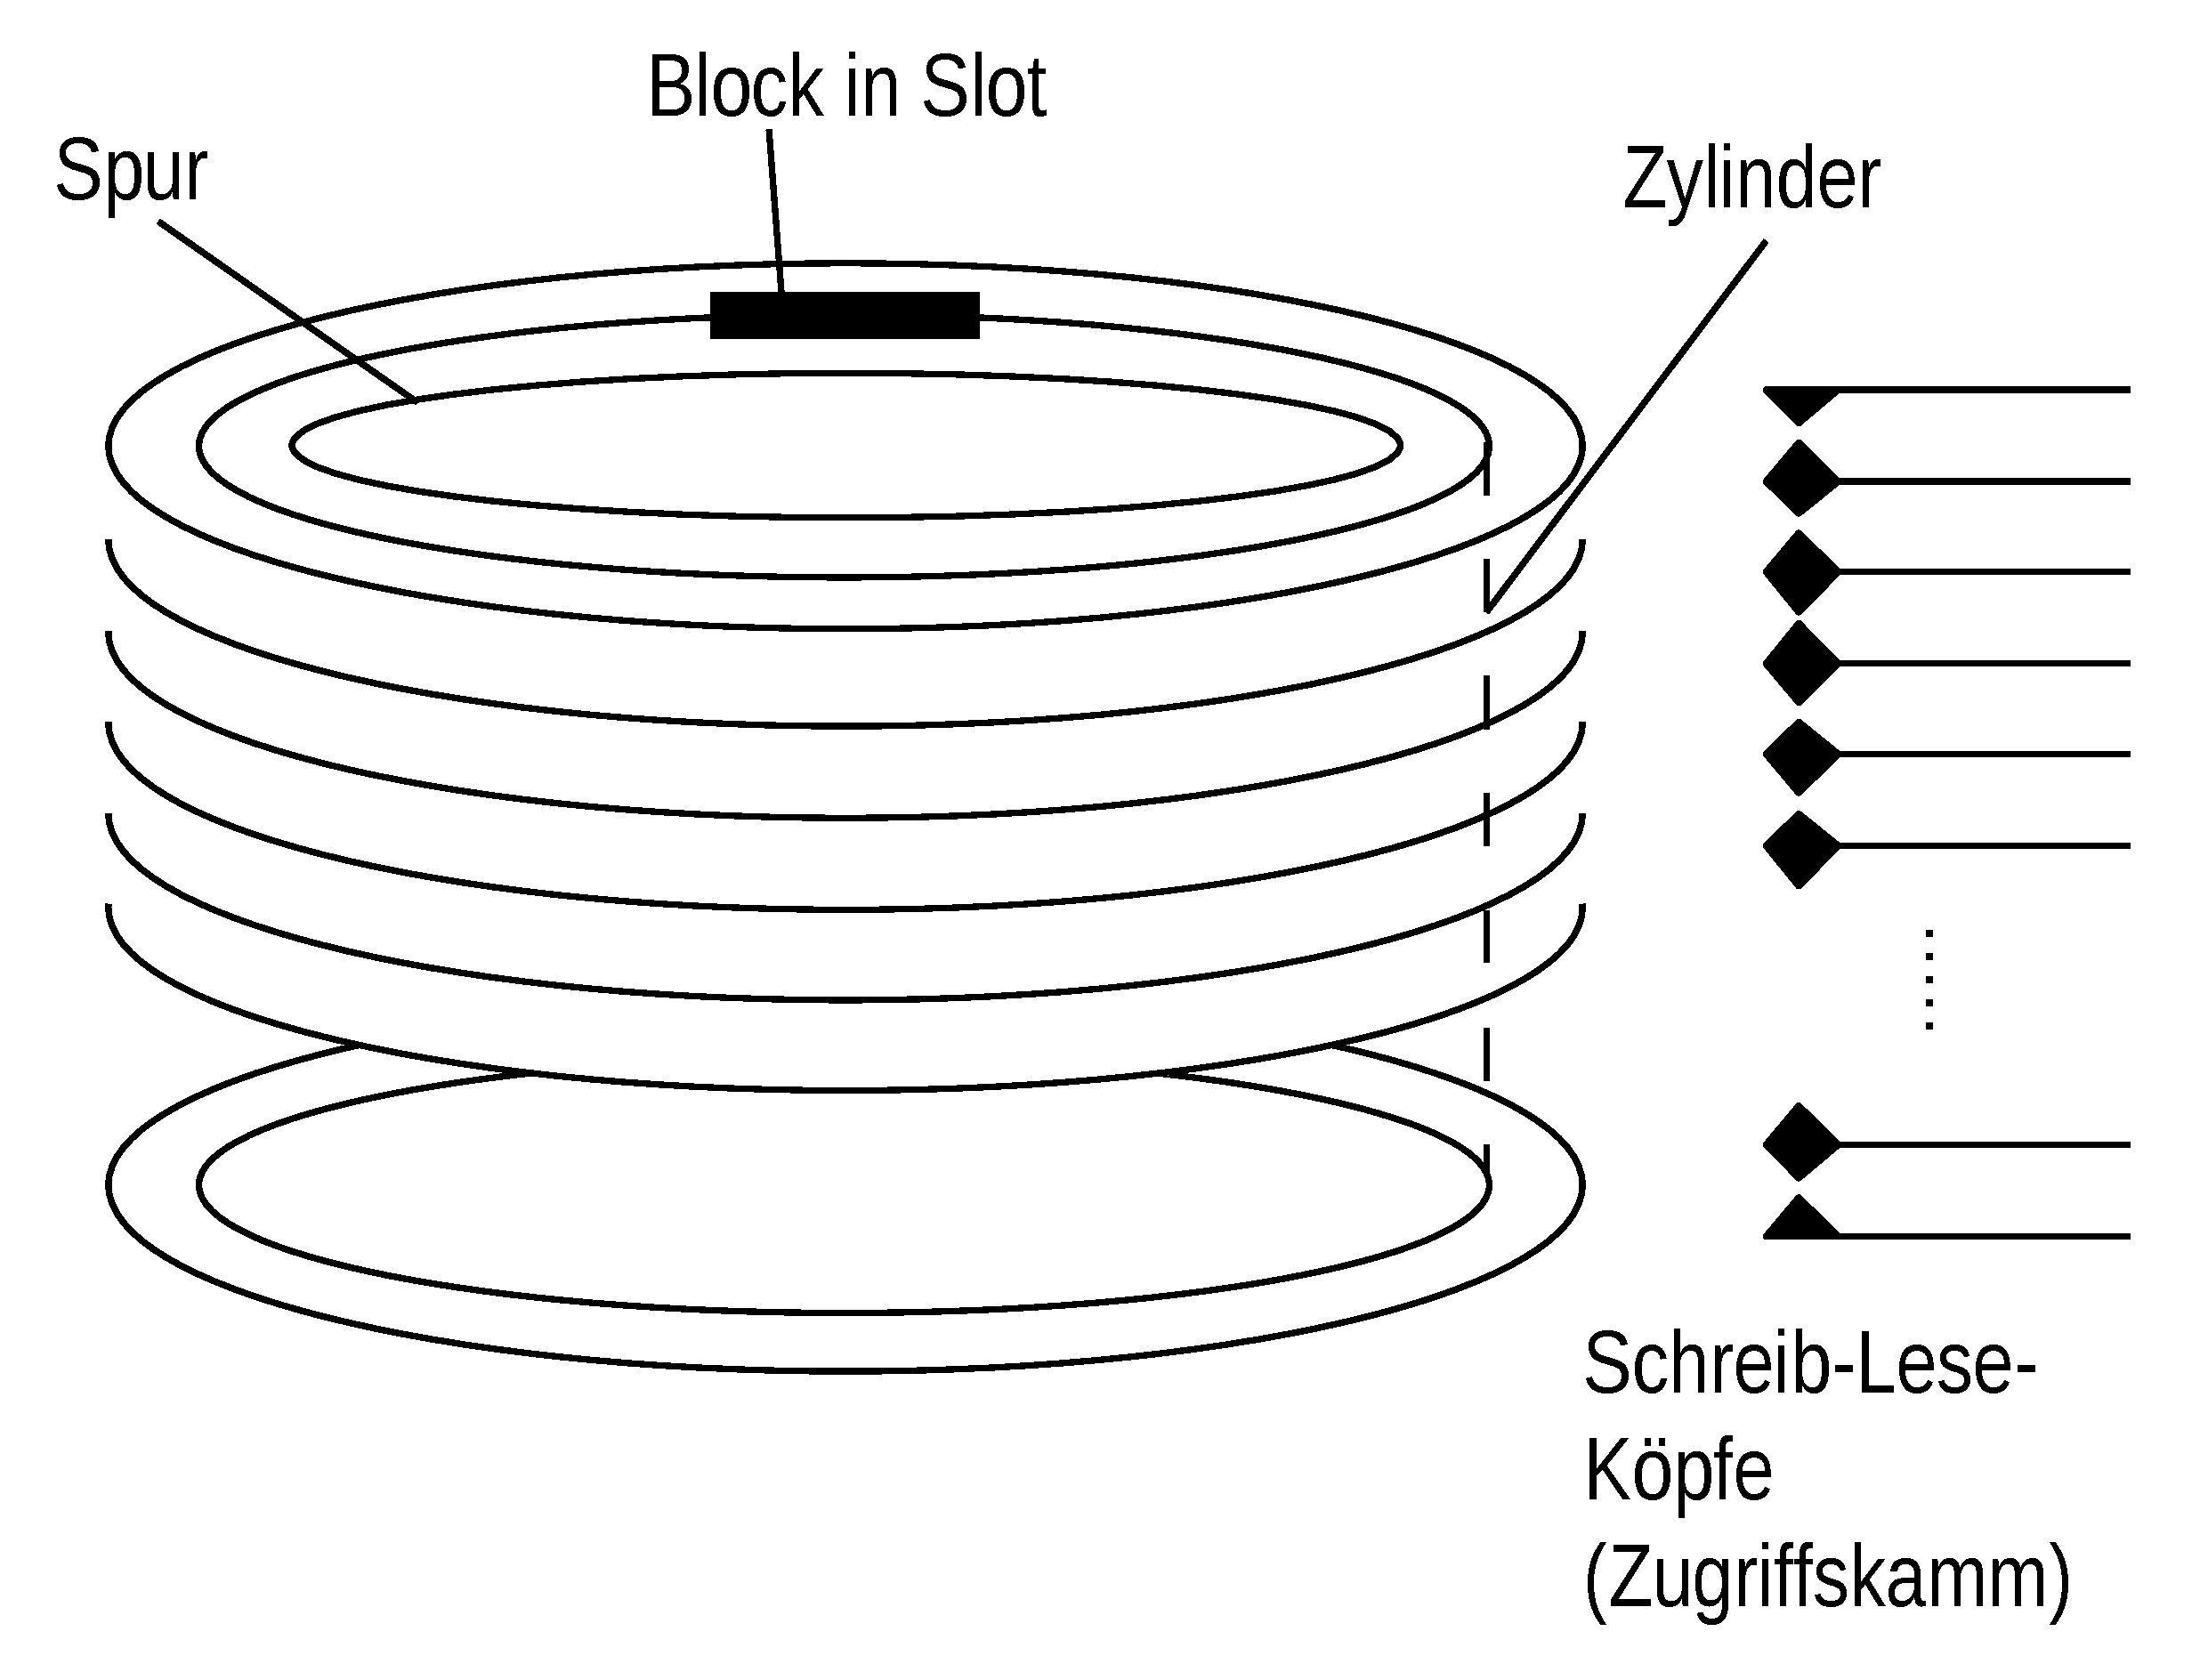
\includegraphics[width=\linewidth]{Pictures/hdd}
	\end{minipage}
	\begin{minipage}{0.49\linewidth}
		Bei einer HDD werden die Blöcke per CHS (\textit{Cylinder}, \textit{Head} (Lesekopf, alternativ \textit{Track} (Spur)), und \textit{Sector} (Slot)) adressiert.
		Der Zugriff auf den ersten Block hat einen hohen Aufwand, da der Lesekopf zunächst auf die richtige Spur ausgerichtet werden muss (Seek-Zeit).
		Anschließend muss (kurz) darauf gewartet werden, bis sich die Platte bis zum richtigen Slot gedreht hat.
		Folgeblöcke aus der selben Spur können dafür aber relativ schnell ausgelesen werden.
		Der Wechsel zu einem anderen Lesekopf/ einer Nachbarspur erfordert ein kurzes Neueinstellen des Zugriffskamms (Track-to-Track-Zeit).
	\end{minipage}
	Bei einer SSD sind die Slots in Speicherchips und Blöcke aufgeteilt.
	Mithilfe mehrerer Speicherchips kann parallel auf das Laufwerk zugegriffen werden.
	Die Blöcke bezeichnen die \textit{kleinste löschbare Einheit}, diese umfasst mehrere Slots und ist meist mehrere Megabyte groß.
	Da das Löschen nur auf dem gesamten Block geschieht wird die  Blockadresse nicht linear auf Slots abgebildet.
	Das Auslesen eines Slots geschieht ohne physische Bewegung, sondern direkt (Leselatenz).
	Sequentielle Zugriffe können zu einem gebündelt werden, wodurch diese beschleunigt werden.
	Weitere Infos zu SSDs können Sie in diesem Blogbeitrag nachlesen: \href{http://databasearchitects.blogspot.com/2021/06/what-every-programmer-should-know-about.html}{databasearchitects.blogspot.com/2021/06/what-every-programmer-should-know-about.html}
\end{solution}

\beamertxt{\pagebreak}
\subsection{Zugriffszeiten}
\label{ZugriffFestplatten}
Stellen Sie sich vor, Sie haben Laufwerke mit folgenden Leistungsdaten:

\begin{minipage}[t]{0.55\linewidth}
	\paragraph{HDD Seagate~Ironwolf~Pro 18~TB (ST18000NE0000)}
	\begin{itemize}
		\item 480.000 Zylinder
		\item 18 Spuren pro Zylinder
		\item 4064 Sektoren pro Spur
		\item 512 Byte pro Sektor
		\item 7200 RPM
		\item Durchschnittliche Latenz: 4.16 ms
		\begin{itemize}
			\item Track-to-Track-Zeit (Annahme): 0,2ms
		\end{itemize}
		\item Kosten 367€ (06/2023)

	\end{itemize}
\end{minipage}
\hfill
\begin{minipage}[t]{0.35\linewidth}
	\paragraph{SSD Seagate FireCuda 530 4TB (ZP4000GM30013)}
	\begin{itemize}
		\item Random Read (Parallel): 1.000.000 IOPS\normaltxt{ (Input / Output Operations Per Second)}, 4KiB Einheiten
		\begin{itemize}
			\item Leselatenz (Annahme): 80µs
		\end{itemize}
		\item Sequential Read: 7300~MB/s, 128~KiB Einheiten
		\item Kosten 377€ (06/2023)
	\end{itemize}
\end{minipage}



\paragraph{Aufgabe}
\begin{enumerate}[a)]
	\item Wie lange benötigen Sie im Mittel, um 10.000 Blöcke (4 KiB, also ca. 39MiB)
	\label{ZugriffFestplattenDauern}

	\begin{enumerate}[i)]
		\item sequentiell zu lesen?

		\begin{solution}
			\begin{description}
				\item[Festplattenlaufwerk]
				\begin{note}
					Evtl vorher berechnen:
					\begin{itemize}
						\item Zeit pro Umdrehung (60s/7200) = 8,33ms
						\item Blöcke pro Spur = 4064/8 = 508
					\end{itemize}
				\end{note}
				Für den Zugriff auf einen beliebigen Slot benötigt es die durchschnittliche Latenz ($T_{Zugriff}$ = 4.16~ms)

				Im Anschluss kann die ganze Spur in $T_{Rotation}$ gelesen werden.
				Doch wie viele Spuren müssen gelesen werden?
				\begin{align*}
					\textit{Blöcke pro Spur} &= \textit{Sektoren pro Spur} / \textit{Sektoren pro Block} = 4064/8 = 508\\ 
					\textit{Anzahl an Spuren} &= \textit{Anzahl an Blöcken} / \textit{Blöcke pro Spur}\\
					&= 10.000 / 508 \approx 19,69
				\end{align*}
				Damit müssen 18 bis 19 volle Spuren und bis zu zwei Spuren anteilig gelesen werden.
				Im einfachsten Fall haben wir eine erste volle Spur, weitere 18 volle Spuren und eine zusätzliche Spur für den Rest.
				Um zwischen 2 benachbarten Spuren zu wechseln fällt keine ganze $T_{Zugriff}$ an, sondern lediglich eine $T_{Track2Track}$.
				Die unvollständige Spur hat in Größe von $10.000 - 19*508 = 348$ Blöcke.
				Damit erhalten wir:
				\begin{align*}
					T_{10.000} &= T_{erste Spur} + 18\cdot T_{ganze Zusätzliche Spur Lesen} + T_{letzte Spur}\\
					&= T_{Zugriff} + T_{Rotation}\\
					&+ 18 (T_{Track2Track}  + T_{Rotation})\\
					&+ T_{Track2Track} + T_{Lesen Letzte Spur}\\
					&= T_{Zugriff} + T_{Lesen Letzte Spur}\\
					&+ 19 (T_{Track2Track}  + T_{Rotation})\\
					&= 4,16ms + 348/508 \cdot 8,33 ms\\
					&+ 19 \cdot (0,2ms + 8,33ms)\\
					&\approx 9,87 + 162,07ms  \approx 172ms
				\end{align*}
				\item[Flashlaufwerk]
				Für 10.000 Blöcke der Größe 4KiB benötigen wir $10.000/(128/4) = 312,5$ also 313 bis 314 Einheiten.
				Wie lange dauert es, eine Einheit zu lesen?
				\begin{align*}
					T_{SequenzielleEinheit} &= 128KiB/7300 MB/s\\
					&= (128 \cdot 1024) /(7300 \cdot 1000\cdot 1000) s  \\
					&\approx 18 \mu s
				\end{align*}
				Damit erhalten wir im schlechtesten Fall $18\mu s \cdot 314 = 5,6ms$
			\end{description}
		\end{solution}


		\item verstreute zu lesen?
		Gehen Sie davon aus, dass die Blöcke völlig zufällig verteilt sind.

		\begin{solution}
			\begin{description}
				\item[Festplattenlaufwerk] 
				Wir gehen in der Musterlösung vom Worst Case aus (= jeder der 10.000 gesuchten Blöcke liegt auf einer anderen zufälligen Spur, was bei 480.000 Spuren nicht unwahrscheinlich ist), d.h. für jeden Block muss $TZugriff$ aufgewendet werden.
				Die Lesezeit für einen Block pro Spur beträgt $1/508$ einer Umdrehung, das ist vernachlässigbar klein.
				Dauer insgesamt: 
				\begin{align*}
					T &= 10000 \cdot ( TZugriff + vernachlaessigbare Lesezeit)\\
					&= 10000 \cdot 4,16ms = 41,6s
				\end{align*}
				\item[Flashlaufwerk]
				Da über jeden NAND-Channel unabhängig zugegriffen werden kann, muss hier der parallele Zugriff vom sequentiellen unterscheiden werden.
				\begin{description}
					\item[sequentiel] Wenn die Blöcke nur einer nach dem anderen zugegriffen werden können, benötigt jeder Block die Leselatenz.
					Damit $10.000\cdot 80\mu s = 800 ms$
					\item[parallel] Beim lesen von 10.000 Blöcken benötigt die SSD jeweils eine IOP.
					Damit $10.000/1.000.000 s = 1/100 s = 10 ms$
				\end{description}
			\end{description}
		\end{solution}

		\begin{note}
			Vielleicht kommt jemand auf die Idee, dass ja rein zufällig zwei Blöcke auf dem gleichen Zylinder liegen.
			Das Geburtstagsparadoxon legt das Nahe.
			Bei insgesamt 10000 Blöcken auf über 480.000 Zylindern (*18 Spuren) liegt die wslkt zwar bei $99,7\% $, jedoch machen bei 10000 Zugriffen eine Hand voll eingesparte Zugriffe auch keinen allzu großen Unterschied.
		\end{note}

	\end{enumerate}




	\item Wie bereits erwähnt, sind SSDs und HDDs unterschiedlich aufgebaut.
	Wie könnte eine einheitliche Schnittstelle aussehen, mit der man Blöcke sowohl von Festplatten als auch von SSDs lesen kann?

	\begin{solution}
		Als gemeinsame Schnittstelle kann man auf jedes Gerät über die Blocknummer zugreifen.
		Das implementieren mit LBA (Logical Block Adressing) auch eigentlich alle Speichermedien seit mindestens 1996 (Win98 ist zwar noch auf 128\,GB beschränkt, aber schon mit LBA).

		Das ist schon eine Abstraktion: Wir müssen nicht mehr das physische Layout der Daten auf einem Laufwerk kennen; wenn wir die Größe eines Gerätes kennen, können wir alle Blöcke adressieren.
		Diese Abstraktion ist notwendig, da neuere Laufwerke (z.B. SSD) einen grundlegend anderen Aufbau als ältere Laufwerke (z.B. HDD) haben.
		Auch HDDs sind unter sich unterschiedlich aufgebaut.
		So kann sich die Anzahl der Zylinder, Spuren pro Zylinder, oder Slots pro Spur beim Austausch einer HDD ändern.
		Gleiches gilt übrigens auch für CDs (constant linear velocity vs. constant angular velocity).
	\end{solution}

	\item Was sind die Vorteile beziehungsweise Nachteile von sehr kleinen und sehr großen Blockgrößen innerhalb eines Dateisystems?

	\begin{solution}
		\paragraph{I/O-Operationen}
		Kleine Blockgrößen haben den Nachteil, dass sehr viele I/O-Operationen notwendig (teuer) sind, was bei großen Blockgrößen deutlich weniger wird.
		Außerdem ist der Verwaltungsaufwand bei kleinen Blöcken größer.
		Dafür ist die Platzverschwendung pro Block nicht so groß.

		\paragraph{Speicherplatz}
		Große Blöcke können Speicherplatzverschwendung sein, da man immer einen ganzen Block allokieren muss.
		Wenn z.B. eine Relation sehr klein ist, nutzt sie nicht den ganzen Block aus.
		Umgekehrt bleibt je Block aber im Mittel der Platz für einen halben Satz ungenutzt.
		Somit verschwenden wir bei kleinen Blöcken weniger Platz.
		Das sehen wir aber erst in der nächsten Übung.
	\end{solution}
	\item Bestimmen Sie die Kosten für die genannten Datenspeicher in $\geneuro/GB$.

	\begin{solution}
		\begin{description}
			\item[HDD] $367\geneuro / 18TB = 367 / (1000*18) \cdot \geneuro/GB \approx 0,02 \geneuro/GB$
			\item[SSD] $377\geneuro / 4TB = 377 /(1000*4) \cdot \geneuro/GB \approx 0,09 \geneuro/GB$
		\end{description}
		Wie Sie erkennen können ist SSD-Speicher um weniger als eine Größeneinheit teurer als HDD-Speicher.
	\end{solution}
\end{enumerate}


\section{Dateiverwaltung}
Welche Operationen müssen in welcher Reihenfolge ausgeführt werden um einen Block einer (blockorientierten) Datei zu lesen?

\begin{enumerate}[\alph{enumi})]
\item Beim öffnen der Datei.
\begin{solution}
\begin{enumerate}
	\item Master File Table bzw. Dateikatalog von der Festplatte über die Gerätesteuerung lesen.
	Dieser Dateikatalog liegt an einer fest definierten Stelle auf der Festplatte.
	\item Solange die angeforderte Datei nicht gefunden wurde, gehe die Hierarchie des Dateikatalogs durch.
	Dies ist abhängig vom Dateisystem (vgl. Vorlesungsfolien~\Katalogeintraege~und SP2).
	\item Überprüfe ob die Zugriffsrechte des Benutzers mit der angeforderten Zugriffsart übereinstimmen.
	\item Lege den Dateikontrollblock für die Datei an.
\end{enumerate}
\end{solution}
\item Beim lesen aus der geöffneten Datei.
\begin{solution}
\begin{enumerate}
	\item Lese aus dem Dateikontrollblock für die Datei die Referenz zum geforderten Block.
	\item Fordere über die Gerätesteuerung den gewünschten Block an.
	\item Die Gerätesteuerung setzt die Blocknummer in den entsprechenden Zugriffsbefehl für den Hintergrundspeicher um und liefert den Block zurück.
	Bei einer HDD beinhaltet dies die Umwandlung der Blocknummer in Slot, Zylinder und Spur.
\end{enumerate}
\end{solution}
\end{enumerate}


\begin{deeper}
\section{Dateizugriff}
Schreiben Sie im Pseudocode die Operation, die einen Block aus einer Datei liest.
Der Dateikatalog soll als Extent-Tabelle gemäß Folie~\KatalogeintraegeVier~im Anhang realisiert sein.
Die Datei kann als bereits geöffnet angenommen werden.
Die Kommunikation mit der Festplatte sei über die Funktion \texttt{readBlock(int CylinderNo, int TrackNo, int SlotNo, ByteBuffer bb)} der Klasse \texttt{Device} zu gestalten.
Die Signatur der Methode \texttt{read} is Folgende: \texttt{void read(int BlockNo, ByteBuffer bb) throws IOException{}}.

\cprotEnv
\begin{note}
\begin{lstlisting}[]
/* Operation
 * int BlockFile::read ( int BlockNo, char *BlockBuffer )
 * wie auf Folie(*@~\textit{\SchreibUndLese}@*)
 */
void read(int BlockNo, ByteBuffer bb) throws IOException {
/* Lesen der Extent-Tabelle auf dem Katalog-Eintrag der
 * (bereits geöffneten) Datei:
 * Extent[i] (Slot-Adresse; AnzSlots)
 * AnzSlots = Zahl der von dieser Adresse an
 * sequenziell belegten Slots
 */
int LocalBlockNo = BlockNo; bool found=false;
// Finde passenden Extent
for(int i = 0; i < Extent.length; i++) {
  if(LocalBlockNo > Extent[i].AnzSlots ) {
    LocalBlockNo -= Extent[i].AnzSlots;
  } else {found=true; break;}
}
if(!found) throw new IOException();
// Startkoordinaten des Extents
int CylinderNo = Extent[i].Slot-Adresse.Zylinder;
int TrackNo = Extent[i].Slot-Adresse.Spur;
int SlotNo = Extent[i].Slot-Adresse.Slot;
// Bewege Koordinaten entsprechend weiter
SlotNo += LocalBlockNo;
/* Überlaufbehandlung: */
while(SlotNo > SlotsPerTrack) {
  SlotNo -= SlotsPerTrack; TrackNo++;
}
while(TrackNo > TracksPerCylinder) {
  TrackNo -= TracksPerCylinder; CylinderNo++;
}
if(CylinderNo > MaxCylinder) throw new IOException();
int Status = Device.readBlock(CylinderNo, TrackNo, SlotNo, bb )
if (Status != 0)  throw new IOException();
return
}
\end{lstlisting}
\end{note}

\end{deeper}

\section{Zugriffsbeschleunigung}
Überlegen Sie sich einige Ideen, wie die Zugriffszeiten auf externe (Online-)Spei\-cher\-me\-di\-en generell verkürzt werden können.

\begin{solution}
\begin{itemize}
	\item Daten gemäß Zylinder organisieren

	Die "`Seek"'-Zeit macht ca. 50\,\% der mittleren Blockzugriffszeit aus. Durch die Platzierung von logisch zusammen gehörenden Daten, deren Kapazität größer als die einer Spur ist, auf dem gleichen Zylinder fällt die "`Seek"'-Zeit beim Lesen im besten Fall nur einmal an.


	\item Verwendung mehrerer Festplatten -- im weitesten Sinne RAID

	Hier gibt es zwei Möglichkeiten:
	\begin{enumerate}
		\item Auf den Platten stehen die gleichen Daten (Spiegelung, Mirroring).
		\item Die verschiedenen Platten enthalten unterschiedliche Daten.
	\end{enumerate}
	In beiden Varianten können sich die Köpfe der Platten unabhängig voneinander bewegen. 	Daher kann man insgesamt mehr seek-Operationen durchführen und außerdem parallel lesen (Durchsatz!).
	In a) klappt das immer, in b) nur dann, wenn die benötigten Daten auf unterschiedlichen 	Platten liegen. Außerdem bietet a) Datensicherheit zum Preis von verschwendetem 	Speicherplatz.
	Das Schreiben kann in b) schneller werden (analog dem Lesen), in a) nicht, da die Daten 	auf alle Platten gleichzeitig geschrieben werden müssen und man nicht parallel 	unterschiedliche Operationen ausführen kann.
Voraussetzung ist natürlich, dass der Disk-Controller dafür ausgelegt ist und Hauptspeicher und Datenbus mit den höheren Transferraten klar kommen.


	\item Scheduling mit Elevator-Algorithmus

	Will man mehrere Zugriffe tätigen, so kann man das evtl. in einer günstigeren Reihenfolge als der angegebenen machen. Eine günstige Reihenfolge ist eine, die die Kopfbewegungen minimiert. Dazu gibt es z.\,B. den sog. Elevator-Algorithmus: man behält die Richtung der Kopfbewegung solange bei, bis in dieser Richtung keine weiteren Aufträge vorliegen. Dabei bearbeitet man immer den nächstgelegenen Auftrag als nächstes. Das tun Festplatten heute schon selbständig. Das Betriebssystem auch.


	\item Prefetching

	Lesen: Wenn man voraussagen kann, welche Blöcke in naher Zukunft gebraucht werden, kann man sie früh (oder. während man sie sowieso passiert) in den Hauptspeicher laden.
	Das funktioniert natürlich nur, wenn die Platte nicht dauerhaft unter Last steht und man 	"`freie Zeit"' zum Prefetching verwenden kann. Für das Lesen "`während man sie sowieso passiert"' braucht man natürlich keine freie Zeit.

	Schreiben: analog

	Sonstige Arten von Pufferung (Caches) zählen wir hier noch nicht, da sie nicht direkt die Zugriffszeiten verringern, sondern gleich die Zugriffe vermeiden.

	\item Komprimierung

	Wenn die Daten auf der Platte effektiv komprimiert wurden, belegen sie weniger Blöcke und können daher schneller in den Hauptspeicher geladen werden. Siehe dazu später auch C-Store (Vorlesung und Übung 9). Jedoch muss im Einzelfall der Geschwindigkeitsvorteil bei der Zugriffszeit dagegen abgewogen werden, dass die Daten vor der Nutzung im Hauptspeicher möglicherweise erst wieder dekomprimiert werden müssen.

\end{itemize}
\end{solution}

\begin{note}
	Eine weitere Idee für die Zugriffsbeschleunigung ist es, die Daten mehrerer Spuren des gleichen Zylinders parallel zu lesen.
	Dies machen moderne Festplatten aber aus praktischen Gründen nicht:

	"`Accessing data in parallel through multiple heads would seem to be an obvious optimization, but it is hard to implement in practice. Before RAID systems became popular, some high performance disks could access data through multiple heads in parallel. These devices required extra read and write electronics, and the heads needed to be aligned with each other very accurately. This was quite difficult because of vibration, thermal gradients, and mechanical imperfections in the drive. As track densities grew, alignment became even more difficult, and the advent of RAID technology has practically eliminated the demand for specialized high performance disk drives. Modern drives access data through only one head at a time."' (John M. May: Parallel I/O for High Performance Computing, 2000, Morgan Kaufmann, S.~19)
\end{note}


\begin{deeper}
\section{Programmieraufgabe 1: Blockfile}

\subsection{Generelles}
Sinn der Programmieraufgabe ist es, im Laufe des Semester eine single-threaded Datenbank selbst zu implementieren.
Die Vorlage, die Sie auf GitLab\footnote{\url{https://gitlab.cs.fau.de/idbprog/vorlage}} herunterladen können, beinhaltet einige Schnittstellen, Hilfsklassen und Testfälle.
Achten Sie darauf, Ihre Implementierung verständlich zu halten, da Sie ggf. im Laufe des Semesters mehrfach bereits gelöste Aufgaben nach versteckten Fehlern durchsuchen müssen.
Wir empfehlen eine Gruppengröße von 2-3 Personen.

Zur Abgabe verwenden wir Git-Repositorys des GitLab der Informatik\footnote{\url{https://gitlab.cs.fau.de}}, auf welche sowohl Sie, als auch die Tutoren Zugriff haben.
Dies erstellen wir für Sie, loggen Sie sich hierfür erstmalig auf der GitLab-Weboberfläche ein und schreiben Sie eine E-Mail mit den Namen und GitLab-Kennungen aller Gruppenmitglieder an \href{mailto:demian.voehringer@fau.de}{demian.voehringer@fau.de}.
Wir empfehlen, dieses auch für Ihre gemeinsame Arbeit zu verwenden.

Die Programmieraufgabe verwendet \textit{ant} und \textit{junit5}.
Sie sollte im CIP direkt funktionieren.
Der CIP dient auch als Referenzsystem, auf dem Ihre Abgabe laufen sollte. %muss.
Zur Übersetzung und Ausführung der \texttt{idb.Main} führen Sie \texttt{ant} in Toplevel aus, für die Testfälle \texttt{ant test}.

Zögern Sie nicht, uns bei Unklarheiten eine Frage im Forum auf StudOn zu stellen.
Mithilfe Ihrer Rückmeldung können die Aufgaben verbessert und Unklarheiten beseitigt werden.
Bitte halten Sie für solche Fragen Ihr Git-Repository auf dem aktuellen Stand, sodass für uns die Möglichkeit besteht, Ihren Code zu betrachten und Ihnen Rückmeldungen zu geben.
%Zusätzlich können Sie sich an die Intensivierungsübung zur Klärung von Fragen wenden.

Die genauen Definitionen sind in den Schnittstellen und durch die Testfälle gegeben.
Ziel ist es, bis zum Ende des Semesters alle Testfälle zu bestehen, wobei ggf. weitere Testfälle während des Semesters entwickelt und an Sie verteilt werden können.
%Zusätzlich schauen wir Stichprobenweise auf die Implementierung, um ein reines Implementieren bis alle Tests klappen zu vermeiden.
%Versuchen Sie auch deswegen einen verständlichen Stil einzuhalten.


Die Aufgaben bestehen aus der Aufgabenstellung und Hinweisen, die bei der Implementierung helfen können.
Die Hinweise sind \textbf{nicht bindend} und als Hilfestellung gedacht, um ein paar übliche Probleme zu vermeiden.
Eine richtige Lösung muss die Hinweise nicht zwingend umsetzen, solange sie die Aufgabenstellung erfüllt.

\subsection{Aufgabenstellung}
\begin{enumerate}
	\item Implementieren Sie eine Klasse, die die Schnittstelle \beamertxt{\linebreak}\texttt{idb.block.BlockFile} implementiert.
		Beachten Sie die Dokumentation der Methoden in der Schnittstelle.
	\item Tragen Sie den Konstruktor Ihrer Klasse in \texttt{idb.construct.Util} in der Methode \texttt{generateBlockFile(int blockSize)} ein.
		\texttt{generateBlockFile(int blockSize)} soll die Blockgröße als Integer aufnehmen und ein neue Blockfile mit dieser Blockgröße zurückgeben.
		Beachten Sie, dass die BlockFile zu diesem Zeitpunkt keine Datei im Dateisystem geöffnet hat.
	\item Sorgen Sie dafür, dass Sie alle Tests aus der Klasse \texttt{BlockTests} erfüllen.
	Sie können diese Testfälle mit \lstinline|ant Meilenstein1| ausführen.
	\item Die Abgabe auf GitLab erfolgt zeitgleich mit der Abgabe der Zusatzaufgaben des nächsten Übungsblattes auf StudOn. Markieren Sie hierfür ihre Abgabe mit dem Tag "`Aufgabe-1"'.
\end{enumerate}

\subsection{Hinweise}
\begin{itemize}
	\item Die Interaktion mit dem Dateisystem aus Java kann in unserem Fall \normaltxt{\linebreak}\texttt{java.io.RandomAccessFile} übernehmen.
	\item Ein \texttt{java.nio.ByteBuffer} ist das, was in Java am ehesten an ein \texttt{char*} aus C herankommt.
		Er übernimmt die Rolle des Speichers, in den die Daten von dem Laufwerk gelesen werden können.
	\item Für diese Aufgabe sind ausschließlich die Klassen in den Paketen \texttt{idb.block} und (zum Testen) \texttt{idb.datatypes} interessant.
		Nutzen Sie diese Aufgabe, um sich mit den Klassen in diesen Paketen vertraut zu machen.
	\item Eine nebenläufige Änderung der Dateigröße im Dateisystem muss nicht beachtet werden.
	\item Seien Sie vorsichtig mit \texttt{RandomAccessFile::read}. \texttt{read} liest nicht n bytes, sondern bis zu n bytes.
		Wenn Sie solange warten möchten, bis alle n bytes vorrätig sind, empfiehlt sich \texttt{readFully}.
	\item Testen Sie Ihre Implementierung, indem Sie den Inhalt der Klasse \texttt{idb.Main} durch Testcode für ihre BlockFile ersetzen.
		Setzen Sie \texttt{Main} auf den orginalen Zustand zurück, sobald Sie sich von der Korrektheit überzeugt haben.
\end{itemize}

\end{deeper}

\end{document}
